%
%	Theorieteil
%

\pagebreak
\section{NIS2 Exploration}

\onehalfspacing

\subsection{Mapping between NIS2 and CIS Controls 8.1}

\subsection{Mapping between NIST SP 800-53 and CIS Controls 8.1}

\subsection{Mapping between NIST SP 800-171 and CIS Controls 8.1}

\subsection{NIS2 Article 21}

The NIS2 directive itself is a legal document organized into Chapters and Articles. It has a pan-European scope and targets critical businesses. NIS2 applies to many entities that provide essential services to the European economy and society, such as Operators of Essential Services (OES) and Digital Service Providers (DSPs). While NIS2 primarily targets medium and large enterprises, smaller entities may still be affected, depending on the services they provide.

As we've seen, much of the content concerns reporting requirements and EU-wide cooperation and institutions, which we will not analyze further in this paper.\footnote{See \textit{EU (2022)}: NIS2 Directive. \cite{nis2}}

Article 21, however, defines the required Cybersecurity risk-management measures for critical infrastructure. In paragraph 2, point (g), NIS2 calls for basic cyber hygiene practices and cybersecurity training.

Any entity covered by the directive must, thus, have an IT Security Policy to implement basic cyber hygiene.\footnote{See \textit{NIS 2 Compliant.org (2024)}: List of Policies Required by NIS 2 Directive. \cite{nisPols}} To strengthen their security postures, entities could rely on one of the major frameworks and standards, such as the NIST SP 800 series, ISO/IEC 27001, Mitre Att\&ck, or CIS Controls.\footnote{See \textit{NIS 2 Compliant.org (2024)}: Requirements Checklist for NIS 2. \cite{nisReqs}}

The directive does not mandate whether an entity chooses one of these frameworks or creates its own policies. It also does not favor or champion any of the mentioned frameworks.

For this paper, we will focus on CIS Controls and the baselines provided by the CIS Benchmarks to fulfill Article 21's requirements.

\subsection{CIS Control 04}

The CIS Controls in the current version (v8) consist of 18 controls:

\begin{enumerate}
    \item Inventory and Control of Enterprise Assets
    \item Inventory and Control of Software Assets
    \item Data Protection
    \item Secure Configuration of Enterprise Assets and Software
    \item Account Management
    \item Access Control Management
    \item Continuous Vulnerability
    \item Audit Log Management
    \item Email and Web Browser Protections
    \item Malware Defenses
    \item Data
    \item Network Infrastructure
    \item Network Monitoring and Defense
    \item Security Awareness and Skills Training
    \item Service Provider
    \item Application Software Security
    \item Incident Response
    \item Penetration Testing\footnote{See \textit{CIS (2024)}: Critical Security Controls v8. \cite{cisControls}}
\end{enumerate}

As with the NIS2 articles, many of these controls are procedural and cannot be automated. Control 04, however, Secure Configuration of Enterprise Assets and Software, is of particular importance for individual IT systems, such as Kubernetes clusters.

Control 04 consists of several subcontrols:

\begin{enumerate}
    \item Establish and Maintain a Secure Configuration Process
    \item Establish and Maintain a Secure Configuration Process for
Network Infrastructure
    \item Configure Automatic Session Locking on Enterprise Assets
    \item Implement and Manage a Firewall on Servers
    \item Implement and Manage a Firewall on End-User Devices
    \item Securely Manage Enterprise Assets and Software
    \item Manage Default Accounts on Enterprise Assets and Software
    \item Uninstall or Disable Unnecessary Services on Enterprise Assets
and Software
    \item Configure Trusted DNS Servers on Enterprise Assets
    \item Enforce Automatic Device Lockout on Portable End-User Devices
    \item Enforce Remote Wipe Capability on Portable End-User Devices
    \item Separate Enterprise Workspaces on Mobile End-User Devices\footnote{See \textit{CIS (2024)}: Critical Security Controls v8 - Control 04. \cite{cisControls}}
\end{enumerate}

Control 4.1 strongly emphasizes the configuration process, as the default configuration for enterprise software is typically geared toward ease of deployment and use rather than security. This is where the CIS Benchmarks come into play.

\subsection{NIS2 Article 21 and CIS Control 04}

Control 4.1 is the prime candidate to support and evaluate NIS2 Article 21 2(g) as it covers basic cyber hygiene and IT security policy.

The requirements in Article 21 are much broader than those of CIS Control 04, but a secure configuration process is a fundamental element.

Fulfilling CIS Control 04 does not imply compliance with Article 21, but noncompliance with CIS Control 04 does imply noncompliance with Article 21.

The CIS Benchmarks can indicate whether an IT system is potentially NIS2 compliant. Evaluating and running the CIS Benchmarks regularly will support NIS2 compliance checking and defense against cyber attacks.

\subsection{CIS Benchmarks on AKS}

Maintaining a Secure Configuration Process is important. Leaving default configurations unchecked might result in some of these security risks:

\begin{itemize}
    \item Exposed Services and Ports
    \item Default Accounts and Passwords
    \item Pre-configured DNS Settings
    \item Older or Vulnerable Protocols
    \item Pre-installed Unnecessary Software\footnote{See \textit{CIS (2024)}: Ibid. \cite{cisControls}}
\end{itemize}

To mitigate these, the CIS Benchmarks provide a security baseline for enterprise software, such as Kubernetes, covering all aspects of CIS Control 4.1 and a matching IT Security Policy.\footnote{See \textit{CIS (2024)}: CIS Benchmarks List. \cite{cisBenchmarks}}

There are CIS Benchmarks tailored to the currently available and supported version of Kubernetes and the major hosted versions, such as the Azure Kubernetes Engine.

\subsection{CIS Benchmarks on RKE2}

\subsection{CIS Kubernetes Benchmark Results}

We'll use the Rancher CIS Scans from above against a simple downstream RKE2 Kubernetes cluster; the Kubernetes Version is v1.28.12+rke2r1, and the CIS Scans application version is v5.3.0.

Running CIS profile 1.8 against our cluster, we receive the following results:

\begin{figure}[H]
\centering
\caption {CIS Scans Results RKE2}
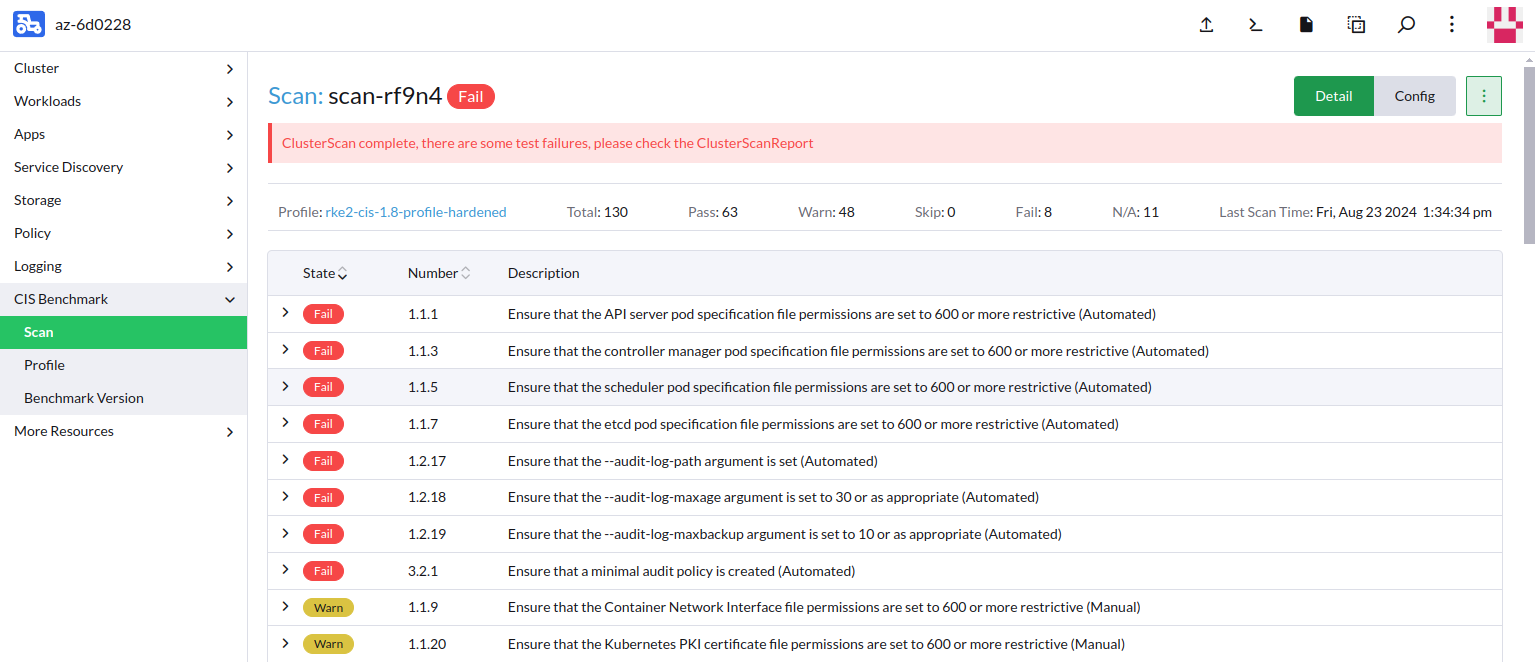
\includegraphics[width=\linewidth]{images/cis-scans-3.png}
\label{fig:cisRKE2}
\end{figure}

Compared to the results from an AKS downstream cluster above, we can see that there are many more failures and warnings. The difference between these two types of clusters, even though they are both Kubernetes v1.28 clusters, is that AKS is a hosted version of Kubernetes. In a hosted version of Kubernetes, the hosting entity provides the control plane, in this case, Microsoft Azure. An RKE2 cluster, however, does include the Kubernetes control plane and thus has a much higher attack surface and many more configuration options.

In the next chapter, we will look at some failures and warnings and possible mitigation steps.
